\documentclass[12pt]{article}
\usepackage[paperwidth=15.5cm, paperheight=8.5cm, margin=0.2cm]{geometry}
\usepackage{tikz}
\usetikzlibrary{positioning, arrows.meta, calc, decorations.pathreplacing}
\pagestyle{empty}
\setlength{\parindent}{0pt}

% ============================================================================
% COLORES Y ESTILOS
% ============================================================================
\definecolor{pastelblue}{RGB}{230, 242, 252}

\tikzset{
  box/.style={
    draw, thick, fill=pastelblue,
    minimum height=1.5cm,
    minimum width=2cm,
    font=\small\sffamily,
    align=center
  },
  ffbox/.style={
    draw, thick, fill=pastelblue,
    minimum width=3.6cm, 
    minimum height=2cm,
    font=\small\sffamily,
    align=center
  },
  signal/.style={-{Stealth[length=2mm]}, thick, black}, 
  wirelabel/.style={font=\tiny\sffamily, text=black, midway, above}
}

% Triangulo de reloj
\newcommand{\clkpin}[1]{
  \draw[thick] ([yshift=-4mm, xshift=0mm]#1.west) -- ++(2.5mm, 2.5mm) -- ++(-2.5mm, 2.5mm);
}

% MUX 2-a-1
\newcommand{\drawmux}[4]{
  \draw[thick, fill=pastelblue] (#1-0.4,#2+0.8) -- (#1+0.4,#2+0.4) -- (#1+0.4,#2-0.4) -- (#1-0.4,#2-0.8) -- cycle;
  \node[font=\tiny\sffamily] at (#1-0.15, #2+0.4) {0};
  \node[font=\tiny\sffamily] at (#1-0.15, #2-0.4) {1};
  \coordinate (#3_in0) at (#1-0.4, #2+0.4);
  \coordinate (#3_in1) at (#1-0.4, #2-0.4);
  \coordinate (#3_in2) at (#1-0.4, #2); 
  \coordinate (#3_out) at (#1+0.4, #2);
  \coordinate (#3_sel) at (#1, #2+0.6);
}

% Adder
\newcommand{\drawadder}[3]{
  \draw[thick, fill=pastelblue] 
    (#1-0.6, #2+1.0) -- 
    (#1-0.6, #2+0.2) -- 
    (#1-0.3, #2) -- 
    (#1-0.6, #2-0.2) -- 
    (#1-0.6, #2-1.0) -- 
    (#1+0.6, #2-0.5) -- 
    (#1+0.6, #2+0.5) -- cycle;
  \node[font=\small\sffamily] (#3) at (#1+0.1, #2) {$+$};
  \coordinate (#3_in1) at (#1-0.6, #2+0.5);
  \coordinate (#3_in2) at (#1-0.6, #2-0.5);
  \coordinate (#3_out) at (#1+0.6, #2);
}

\begin{document}
\noindent
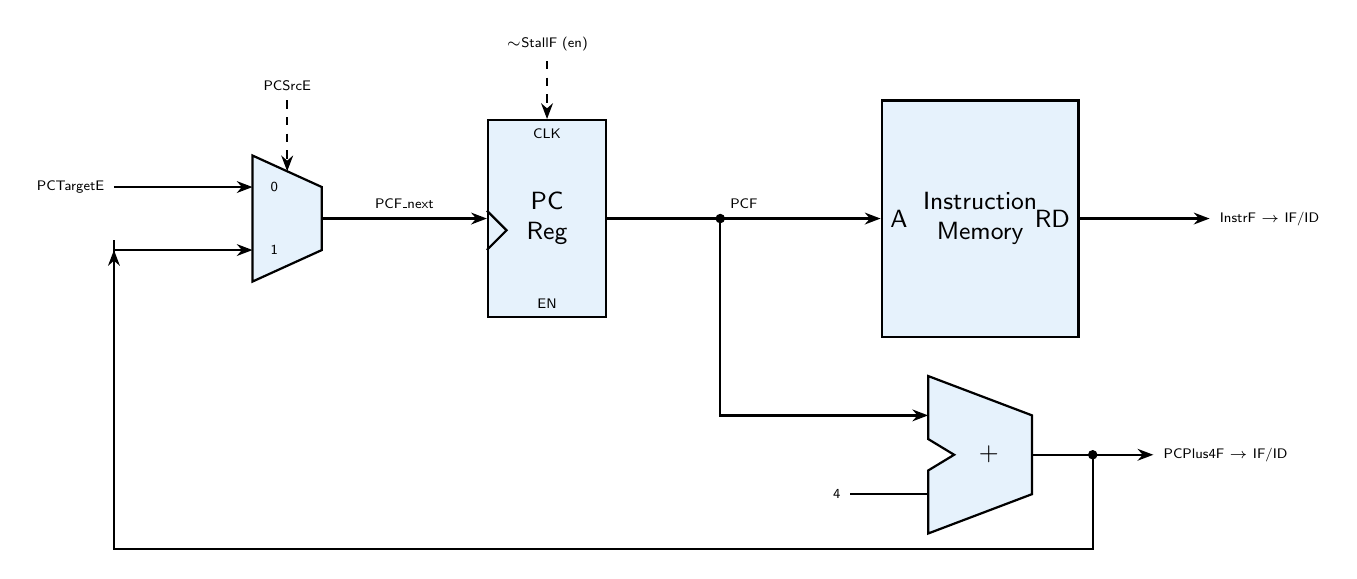
\begin{tikzpicture}[
  x=1.1cm, y=1.0cm,
  signal/.style={-{Stealth[length=2mm]}, thick, black},
  lbl/.style={font=\tiny\sffamily, text=black},
  lblcenter/.style={font=\small\sffamily, align=center},
]

% MUX y PC (MUX en x=0, y=1.0)
\drawmux{0}{1}{pcmux}{MUX PC}

\node[box, minimum height=2.5cm, minimum width=1.5cm] (pcreg) at (3, 1) {};
\node[lblcenter] at (3, 1) {PC\\Reg};
\clkpin{pcreg}
\node[font=\tiny\sffamily, below] at (pcreg.north) {CLK};
\node[font=\tiny\sffamily, above] at (pcreg.south) {EN};

% Memoria (en x=8, y=1.0)
\node[box, minimum height=3cm, minimum width=2.5cm] (imem) at (8, 1) {};
\node[lblcenter] at (8, 1) {Instruction\\Memory};
\node[font=\small\sffamily, right] at (imem.west |- {0,1}) {A};
\node[font=\small\sffamily, left] at (imem.east |- {0,1}) {RD};

% Adder (en x=8, y=-2.0)
\drawadder{8}{-2}{add4}

% Conexiones
% PCTargetE viene de Execute (a la izquierda para modularidad)
\draw[signal] (-2.0, 1.4) -- (pcmux_in0);
\node[left, lbl] at (-2.0, 1.4) {PCTargetE};

% Feedback PCPlus4F entra al Mux por la entrada 1 (y=0.6)
\draw[signal] (-2.0, 0.6) -- (pcmux_in1);

% MUX a PC Reg
\draw[signal] (pcmux_out) -- (pcreg.west) node[midway, above, lbl] {PCF\_next};

% PC Reg a Imem Address
\draw[signal] (pcreg.east) -- (imem.west |- {0,1}) node[midway, above, lbl] {PCF};

% Tap de PCF al Adder entrada 1 (add4_in1 está en 7.4, -1.5)
\draw[fill=black] (5.0, 1.0) circle (1.5pt);
\draw[signal] (5.0, 1.0) |- (add4_in1);

% Adder entrada 2 (constante 4)
\draw[thick] (6.5, -2.5) -- (add4_in2);
\node[left, lbl] at (6.5, -2.5) {4};

% Adder salida (add4_out está en 8.6, -2.0)
\draw[signal] (add4_out) -- ++(1.4, 0) node[right, lbl] {PCPlus4F $\rightarrow$ IF/ID};

% Lazo de realimentación ortogonal
\draw[fill=black] (9.3, -2.0) circle (1.5pt);
\draw[signal] (9.3, -2.0) |- (9.3, -3.2) -- (-2.0, -3.2) |- (-2.0, 0.6);

% Instrucción de salida
\draw[signal] (imem.east |- {0,1}) -- ++(1.5, 0) node[right, lbl] {InstrF $\rightarrow$ IF/ID};

% Líneas de Control (dashed)
\draw[signal, dashed] (0.0, 2.5) node[above, lbl] {PCSrcE} -- (pcmux_sel);
\draw[signal, dashed] (3.0, 3.0) node[above, lbl] {$\sim$StallF (en)} -- (pcreg.north);

\end{tikzpicture}
\end{document}
